\chapter{Markov Chain Solutions}
	\section{Damage Distributions}
		Under \textit{standard} conditions, an attacker's damage distribution, given by $\{c_i\}$ is a uniform distribution from 1 to their max hit with some additional weighting on 0 due to accuracy. This can be generalized to arbitrary probability distributions, allowing consideration of special equipment (like Keras, Verac's, etc.) as well as combining distributions in the case of multiple opponents/attacks. To describe this, we define the following terms:
		\begin{align}
		c_i & \text{ is the probability of doing $i$ damage} \\
		c_0 & \text{ is the probability of doing zero damage} \\
		c_+ &= 1 - c_0 \text{ is the probability of doing damage} \\
		m & \text{ is the largest non-zero probability from $c_i$} \\
		&\text{No healing allowed.}
		\end{align}

		Damage distributions are generally defined as any probability distribution, although in practice the in-game distributions come from a fixed set, as described in Fig.~\ref{fig:damage_distributions}. The suggestion here is that damage distributions constitute an additional dimension for the developers to use (previously only max hit and accuracy were the only parameters). Since this suggestion several items have emerged with special damage distributions (eg: \href{https://oldschool.runescape.wiki/w/Osmumten%27s_fang}{Osmumten's fang}). The math further suggests variable weapon attack speeds as a way of generalizing the integer time steps. This is reflected in new weapons which strike twice (\href{https://oldschool.runescape.wiki/w/Dual_macuahuitl}{eg: Dual Macuahuitl}), and in which delays are added. 


		\begin{figure}
		\centering
		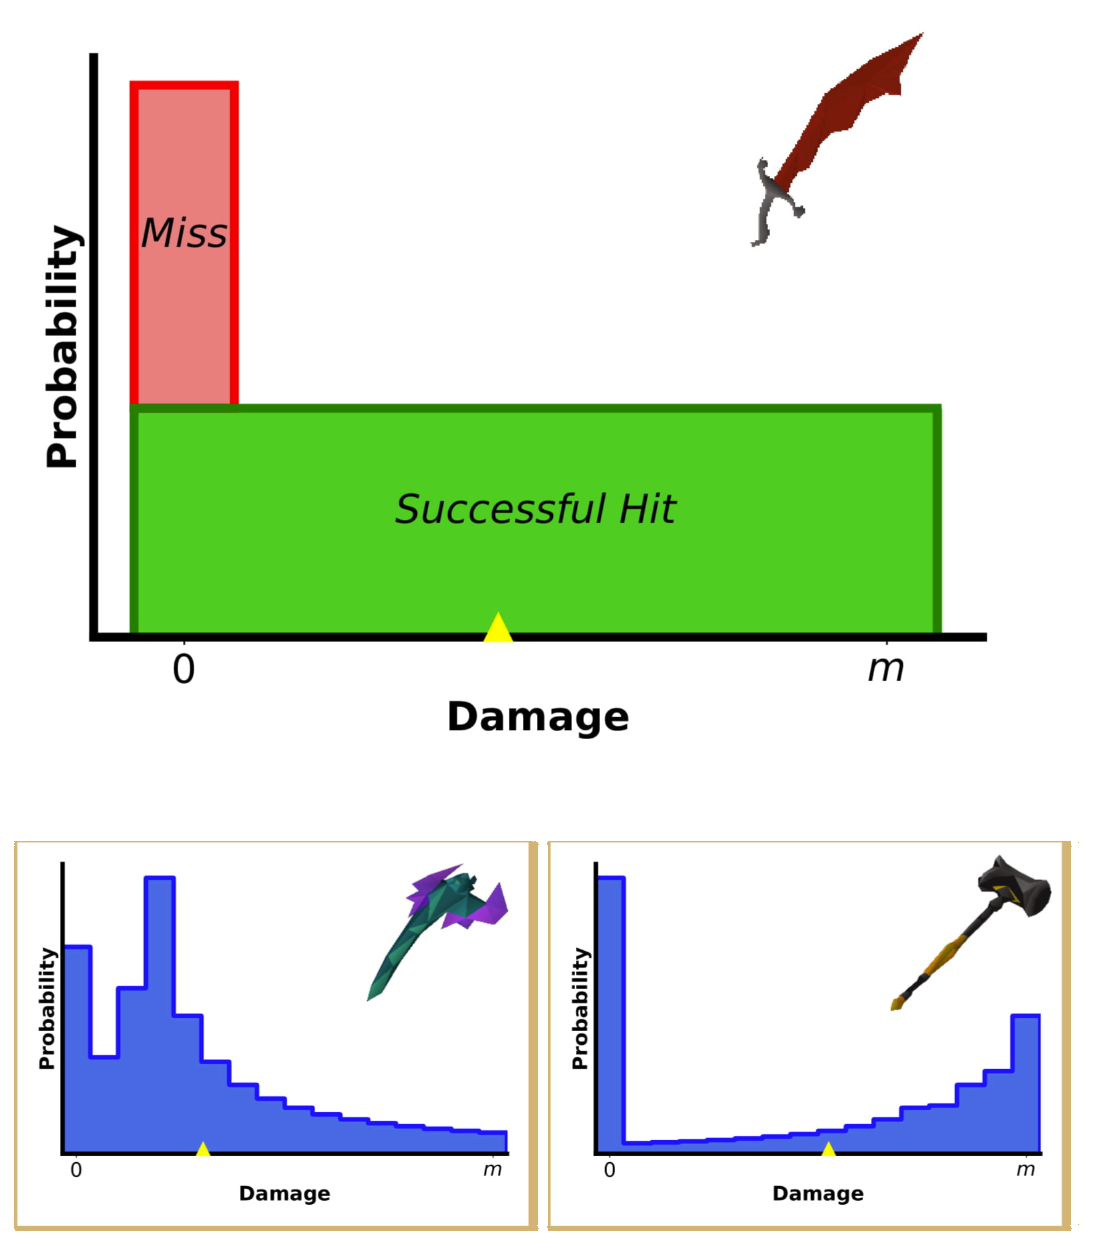
\includegraphics[width=\linewidth]{img/combat/damage_distributions.png}
		\caption{
			The standard damage distribution is shown on top, which consists of a portion to hit successfully and a chance to miss (both based on the accuracy roll). Although the developers modified this distribution in 2024 to enforce that successful hits do at least 1 damage, thankfully all the mathematics still follows (showcasing the benefit of a general solution!). In the bottom are theoretical distributions of hypothetical weapons. On the left, a quick firing weapon has a high chance to do low damage. On the right, a huge maul misses very often but when it hits the damage is very high. Other distributions already exist in-game like the scythe which has a Gaussian distribution and Keras which are considered as two merged distributions. 
		}
		\label{fig:damage_distributions}
	\end{figure}

	\section{Recursive Equation}
	In one attack, the opponent can be brought to a given health $i$, from their initial health $h$ according to the transition probability, \cite{nukelawe:osrs-markov}
	\begin{align}
		\pi_{h, i} &= \begin{cases}
			P(X=h - i) & \text{if } i > 0 \\
			P(X \ge h) & \text{if } i = 0.
	    \end{cases}
	\end{align}
	The probability they are killed in $L$ turns can be given by the sum of the probabilities the opponent was brought to $i$, then killed in $L - 1$ turns:
	\begin{align}
		P_{h, L} &= \sum_{i=0}^\infty \pi_{h, i} P_{i, L-1}\\
		&= \cancel{\pi_{h, 0} P_{0, L-1}} + \pi_{h, h} P_{h, L-1} + \sum_{i=1}^{h-1} \pi_{h, i} P_{i, L-1} + \sum_{i=h+1}^\infty \pi_{h, i} P_{i, L-1}\\
		&= c_0P_{h, L-1} + \sum_{i=1}^{h-1} \pi_{h, i} P_{i, L-1} + \cancel{\sum_{i=h+1}^\infty \pi_{h, i} P_{i, L-1}}\\
		P_{h, L} &= c_0P_{h, L-1} + \sum_{i=\max(h-m, 1)}^{h-1} c_{h-i} P_{i, L-1}\\
	\end{align}
	where in the second line, the $i=0, h$ terms are explicitly considered, and the remaining sum is split in two. In the third line, $\pi_{h, i}$ would correspond to healing which we are taking to be zero. In the final line, we get the lower bound by considering that 
	\begin{align}
		1\leq i \leq h-1 \implies& \pi_{h, i} = c_{h-i} \text{ if } 1\leq h - i \leq m \text{ otherwise } 0,\,\,\, \\
		\implies& 1\leq h - i \text{ and } h - i \leq m\\
		&\therefore  i\leq h - 1 \text{ and } h - m \leq i.
	\end{align}
	Since the first condition is already met, we have that $i \geq h - m$, but $i$ also cannot be below 1, hence $i\geq \max(h - m, 1)$. 



	\section{Solution}
		The recursive equation to solve is:
		\begin{align}
			P_{h, L} &= c_0P_{h, L - 1} + \sum_{i\in I_h} c_{h-i} P_{i, L-1},\,\,\, L \ge 2, h \ge 1\\ % maybe 2
		\end{align}
		where $I_h$ is the set of integers satisfying $h - 1 \ge i \ge \max(h - m, 1)$. The boundary conditions are given by:
		\begin{align}
			P_{h, 1} &= \sum_{i=h}^m c_i \text{ (P of doing more than h damage)} \\
			 &= \theta(m - h) \sum_{i=h}^m c_i \\
			P_{1, L} &= c_+ c_0^{L-1} \text{ (P of missing $L-1$ times, then hitting any damage}\\
			P_{1, 1} &= c_+ \text{ (P of doing any damage)}
		\end{align}
		
		Using a generating function:
		\begin{align}
			g(x, y) &= \sum_{h=1}^\infty\sum_{L=1}^\infty P_{h, L} y^h x^L \\
			&= \sum_{h=1}^\infty\left(P_{h, 1} y^h x + \sum_{L=2}^\infty P_{h, L} y^h x^L \right)\\
			&= \sum_{h=1}^\infty P_{h, 1} y^h x + \sum_{h=1}^\infty\sum_{L=2}^\infty P_{h, L} y^h x^L\\
			&= xyP_{1, 1} + \sum_{h=2}^\infty P_{h, 1} y^h x + \sum_{L=2}^\infty\left( P_{1,L} yx^L + \sum_{h=2}^\infty P_{h, L} y^h x^L \right)\\
			&= xyP_{1, 1}  + x\sum_{h=2}^\infty P_{h, 1} y^h + \sum_{L=2}^\infty P_{1,L} yx^L + \sum_{L=2}^\infty\sum_{h=2}^\infty P_{h, L} y^h x \\
			&= xyP_{1, 1}  + x\sum_{h=2}^\infty P_{h, 1} y^h  + y\sum_{L=2}^\infty P_{1,L} x^L + \sum_{L=2}^\infty\sum_{h=2}^\infty P_{h, L} y^hx^L
		\end{align}
		These are the boundaries of a grid (corner $+$ top $+$ left) plus a sum over the interior. 

		% \subsection{Corner} 
		% Let's focus on each term at a time, starting with the corner:
		% \begin{align}
		% 	xyP_{1, 1} = xyc_+
		% \end{align}
		% \subsection{Top}
		% For the top, lets first note that $\max(m - h + 1, 0)$ is non-zero when $m - h + 1 \ge 1 \implies m \ge h$. Then,
		% \begin{align}
		% 	x\sum_{h=2}^\infty P_{h, 1} y^h &= x \sum_{h=2}^\infty \theta(m - h)\sum_{i=h}^m c_i y^h\\
		% 	&= x\sum_{h=2}^m \sum_{i=h}^m c_i y^h
		% \end{align}
		% \subsection{Left}
		% Now the left:
		% \begin{align}
		% 	y\sum_{L=2}^\infty P_{1,L} x^L &= y\sum_{L=2}^\infty c_+ c_0^{L-1} x^L \\
		% 	&= y\frac{c_+}{c_0}\sum_{L=2}^\infty (c_0x)^L \\
		% 	&= y\frac{c_+}{c_0}\left[\sum_{L=0}^\infty (c_0x)^L - 1 - c_0x\right]\\
		% 	&= y\frac{c_+}{c_0}\left[\frac{1}{1-c_0x} - 1 - c_0x\right]\\
		% 	&= y\frac{c_+}{c_0}\frac{1}{1-c_0x}\left[1 - (1-c_0x) - (1-c_0x)c_0x\right]\\
		% 	&= y\frac{c_+}{c_0}\frac{1}{1-c_0x}\left[c_0^2x^2\right]\\
		% 	&= y\frac{c_+}{c_0}\frac{c_0^2x^2}{1-c_0x}
		% \end{align}
		\subsection{Interior}
		Let's first tackle the interior:
		\begin{align}
			\sum_{L=2}^\infty\sum_{h=2}^\infty P_{h, L} y^hx^L &= \sum_{L=2}^\infty\sum_{h=2}^\infty \left(c_0P_{h, L - 1} + \sum_{i\in I_h} c_{h-i}P_{i, L-1}\right) y^hx^L\\
			&= \sum_{L=2}^\infty\sum_{h=2}^\infty c_0P_{h, L - 1}y^hx^L + \sum_{L=2}^\infty\sum_{h=2}^\infty\sum_{i\in I_h} c_{h-i}P_{i, L-1}y^hx^L\\
			\mathcal{I}(x, y)&= G(x, y) + R(x, y).
		\end{align}
		Let us also tackle this individually, starting with the $G$ term:
		\begin{align}
			G(x, y) = \sum_{L=2}^\infty\sum_{h=2}^\infty c_0P_{h, L - 1}y^hx^L &= c_0\sum_{L=1}^\infty\sum_{h=2}^\infty P_{h, L}y^hx^{L+1}\\
			&= c_0x\sum_{L=1}^\infty\sum_{h=2}^\infty P_{h, L}y^hx^L\\
			&= c_0x\sum_{L=1}^\infty\left( \sum_{h=1}^\infty P_{h, L}y^hx^L -  P_{1, L}yx^L\right)\\
			&= c_0x\sum_{L=1}^\infty\sum_{h=1}^\infty P_{h, L}y^hx^L -  c_0xy\sum_{L=1}^\infty P_{1, L}x^L\\
			&= c_0xg(x, y) -  c_0xy\sum_{L=1}^\infty P_{1, L}x^L\\
			% &= c_0xg(x, y) -  c_+ c_0xy\sum_{L=1}^\infty c_0^{L-1}x^L\\
			% &= c_0xg(x, y) -  c_+ c_0x^2y\sum_{L=1}^\infty c_0^{L-1}x^{L-1}\\
			% &= c_0xg(x, y) -  c_+ c_0 x^2y \sum_{L=0}^\infty c_0^{L}x^L\\
			% &= c_0xg(x, y) -  \frac{c_+ c_0x^2y}{1-c_0x}\\
			% &= c_0xg(x, y) -  y\frac{c_+}{c_0}\frac{c_0^2x^2}{1-c_0x}
		\end{align}
		
		% Followed by $R$. 
		% First let's note that $I$ is a non-empty set when $h-1>=\max(m-h, 1)$, empirically this is equivalent to:
		% $$h\ge \max\left(\left\lceil \frac{m + 1}{2} \right\rceil, 2\right)\equiv M \ge 2$$
		For $R$, we will first need a term that tells us whether $h$ is in the set $I$, i.e. does $h$ satisfy $h-1>=\max(m-h, 1)$? You will actually see that we need the more general $h-1>=\max(m-h+n, 1)$. We will call this condition $\delta_{m, h}^n$ which is $1$ if satisfied and $0$ otherwise. Empirically, this can be expressed as:
		\begin{align}
			\delta_{m, h}^n = \begin{cases}
				0 & \text{ if } h = 1 \\
				0 & \text{ if } n > m \\
				1 & \text{ otherwise }
			\end{cases}
		\end{align}
		Since $h >=2$,
		\begin{align}
			\delta_{m, h}^n = \delta_m^n = \begin{cases}
				1 & \text{ if } n \le m\\
				0 & \text{ otherwise }
			\end{cases}
		\end{align}

		Now solving $R(x, y)= \sum_{L=2}^\infty\sum_{h=2}^\infty\sum_{i\in I} c_{h-i}P_{i, L-1}y^hx^L$ gives:
		\begin{align}
			R(x, y) &= \sum_{L=2}^\infty\sum_{h=2}^\infty\sum_{i=\max(h-m, 1)}^{h-1} c_{h-i}P_{i, L-1}y^hx^L\\
			&= x \sum_{L=1}^\infty\sum_{h=2}^\infty\sum_{i=\max(h-m, 1)}^{h-1} c_{h-i}P_{i, L}y^hx^L\\
			&= xy \sum_{L=1}^\infty\sum_{h=1}^\infty\sum_{i=\max(h-m+1, 1)}^{h} c_{h-i}P_{i, L}y^hx^L\\
			&= xy \sum_{L=1}^\infty\sum_{h=1}^\infty\left(c_0P_{h, L}\delta_m^1 + \sum_{i=\max(h-m+1, 1)}^{h-1} c_{h-i}P_{i, L}\right)y^hx^L\\
			&= c_0xy \sum_{L=1}^\infty\sum_{h=1}^\infty P_{h, L}x^L\delta_m^1 + xy \sum_{L=1}^\infty\sum_{h=1}^\infty\sum_{i=\max(h-m+1, 1)}^{h-1} c_{h-i}P_{i, L}y^hx^L\\
		\end{align}
			\textcolor{red}{This part is outdated/incomplete, each $y$ should have a $c$.}
		Notice that the $h=1$ term in the second set of sums yields 0.
		\begin{align}
			&= c_0 xy g(x, y)\delta_h^1 + xy \sum_{L=1}^\infty\sum_{h=2}^\infty\sum_{i=\max(h-m+1, 1)}^{h-1} c_{h-i}P_{i, L}y^hx^L\\
			&= c_0xy g(x, y)\delta_h^1 + xy^2 \sum_{L=1}^\infty\sum_{h=1}^\infty\sum_{i=\max(h-m+2, 1)}^{h} c_{h-i}P_{i, L}y^hx^L\\
			&= c_0xy g(x, y)\delta_h^1 + xy^2 \sum_{L=1}^\infty\sum_{h=1}^\infty\left(\sum_{i=\max(h-m+2, 1)}^{h} c_{h-i}P_{i, L}\right)y^hx^L\\
			&= c_0xy g(x, y)\delta_h^1 + xy^2 \sum_{L=1}^\infty\sum_{h=1}^\infty\left(P_{i, L}\delta_m^2 + \sum_{i=\max(h-m+2, 1)}^{h} c_{h-i}P_{i, L}\right)y^hx^L\\
			&= c_0xy g(x, y)\delta_h^1 + xy^2 \sum_{L=1}^\infty\sum_{h=1}^\infty P_{i, L}\delta_m^2 + c_+xy^2 \sum_{L=1}^\infty\sum_{h=1}^\infty\sum_{i=\max(h-m+2, 1)}^{h} c_{h-i}P_{i, L}y^hx^L\\
			&= c_0xy g(x, y)\delta_h^1 + xy^2 g(x, y)\delta_m^2 + xy^2 \sum_{L=1}^\infty\sum_{h=1}^\infty\sum_{i=\max(h-m+2, 1)}^{h} c_{h-i} P_{i, L}y^hx^L\\
		\end{align}
		These series continues until the `engine' producing terms has no more. The number of terms in this series is given by the maximum $n$ that is non-zero:
		\begin{align}
			\arg \max_n \delta_m^n = m,
		\end{align}
		and so,
		\begin{align}
			R(x, y) &= x g(x, y)\sum_{i=1}^m c_i y^i
		\end{align}
		% Followed by the recursive term (you'll see where it gets the name):
		% \begin{align}
		% 	c_+ \sum_{L=2}^\infty\sum_{h=2}^\infty\sum_{i\in I} P_{i, L-1}y^hx^L &= c_+ \sum_{L=1}^\infty\sum_{h=2}^\infty\sum_{i\in I_h} P_{i, L}y^hx^{L+1}\\
		% 	&= c_+ \sum_{h=2}^\infty\sum_{L=1}^\infty\sum_{i\in I_h} P_{i, L}y^hx^{L+1}\\
		% 	&= c_+ x\sum_{L=1}^\infty\sum_{h=2}^\infty\sum_{i\in I_h} P_{i, L}y^hx^L\\
		% 	&= c_+ x\sum_{L=1}^\infty x^L\left[\sum_{h=2}^\infty \sum_{i=\max(m-h, 1)}^{h-1} P_{i, L}y^h\right]\\
		% 	&= c_+ x\sum_{L=1}^\infty x^L\left[y\sum_{h=1}^\infty \sum_{i=\max(m-h-1, 1)}^{h} P_{i, L}y^h\right]\\
		% 	&= c_+ x\sum_{L=1}^\infty x^L\left[y\sum_{h=1}^\infty \left(P_{h, L}y^h + \sum_{i=\max(m-h-1, 1)}^{h-1} P_{i, L}y^h \right)\right]\\
		% 	&= c_+ x\sum_{L=1}^\infty x^L\left[y\sum_{h=1}^\infty P_{h, L}y^h + y\sum_{h=1}^\infty\sum_{i=\max(m-h-1, 1)}^{h-1} P_{i, L}y^h \right]\\
		% 	&= c_+ xy\sum_{L=1}^\infty \sum_{h=1}^\infty P_{h, L}y^hx^L + c_+ xy\sum_{L=1}^\infty x^L\sum_{h=1}^\infty\sum_{i=\max(m-h-1, 1)}^{h-1} P_{i, L}y^h \\
		% 	&= c_+ xyg(x, y) + c_+ xy\sum_{L=1}^\infty \sum_{h=1}^\infty\sum_{i=\max(m-h-1, 1)}^{h-1} P_{i, L}y^hx^L \\
		% 	&= c_+ xg(x, y) \left(y + y^2 + ...\right) \\
		% 	&= c_+ xg(x, y) \frac{1}{1-y} \\
		% \end{align}
		Now let's combine everything:
		\begin{align} 
			% g(x, y) &= xyc_+ + x \sum_{h=2}^m \sum_{i=h}^{m}c_i y^h + \cancel{y\frac{c_+}{c_0}\frac{c_0^2x^2}{1-c_0x}} + c_0xg(x, y) - \cancel{y\frac{c_+}{c_0}\frac{c_0^2x^2}{1-c_0x}} +  x g(x, y)\sum_{i=1}^m c_{i} y^i\\
			% &= x \sum_{h=1}^m\sum_{i=h}^{m}c_i y^h + c_0xg(x, y) + x g(x, y)\sum_{i=1}^m c_{i} y^i
			g(x, y) &= xyP_{1,1} + x\sum_{h=2}^\infty P_{h,1}y^h + y\sum_{L=2}^\infty P_{1, L}x^L + c_0xg(x, y) - c_0xy\sum_{L=1}^\infty P_{1, L}x^L + xg(x, y)\sum_{i=1}^m c_iy^i\\
			&= xyP_{1,1} + x\sum_{h=2}^\infty P_{h,1}y^h + \left(y\sum_{L=2}^\infty P_{1, L}x^L - c_0xy\sum_{L=1}^\infty P_{1, L}x^L\right) + xg(x, y)\sum_{i=0}^m c_iy^i\\
			&= x\sum_{h=1}^\infty P_{h,1}y^h + y\left(\sum_{L=2}^\infty P_{1, L}x^L - c_0\sum_{L=1}^\infty P_{1, L}x^{L+1}\right) + xg(x, y)\sum_{i=0}^m c_iy^i\\
			&= x\sum_{h=1}^\infty P_{h,1}y^h + y\left(\sum_{L=2}^\infty P_{1, L}x^L - c_0\sum_{L=2}^\infty P_{1, L-1}x^L\right) + xg(x, y)\sum_{i=0}^m c_iy^i\\
			&= x\sum_{h=1}^\infty P_{h,1}y^h + y\sum_{L=2}^\infty \left(P_{1, L}x^L - c_0P_{1, L-1}\right)x^L + xg(x, y)\sum_{i=0}^m c_iy^i\
		\end{align}
		Here, we will make a simplifying assumption that
		\begin{align}
			P_{1, L}x^L = c_0P_{1, L-1},\,\,\,L\ge2
		\end{align}
		which is the condition that [killing an opponent] in $L$ turns is done by missing once then killing them in $L-1$ turns. This does \emph{not} hold if healing is allowed. Under this assumption we are left with:
		\begin{align}
			g(x, y) &= x\sum_{h=1}^\infty P_{h,1}y^h + xg(x, y)\sum_{i=0}^m c_iy^i\\
			g(x, y) - xg(x, y)\sum_{i=0}^m c_iy^i &= x\sum_{h=1}^\infty P_{h,1}y^h\\
			g(x, y)\left[1 - x\sum_{i=0}^m c_iy^i \right] &= x\sum_{h=1}^\infty P_{h,1}y^h\\
			g(x, y) &= \frac{x\sum_{h=1}^\infty P_{h,1}y^h}{1 - x\sum_{i=0}^m c_iy^i}
		\end{align}
		To simplify, let's define:
		\begin{align}
			T(x) &\equiv \sum_{h=1}^\infty P_{h, 1} y^h \equiv \sum_{h=1}^m t_h y^h \\
			B(y) &\equiv \sum_{i=0}^m c_i y^i,
		\end{align}
		Now $g(x, y)$ can be written as,
		\begin{align}
			g(x, y) &= \frac{xT(y)}{1- B(y)x}.
		\end{align}

		\subsection{Obtaining Power Series}

		Let us start with:
		\begin{align}
			\frac{1}{1- B(y)x} &= \sum_{k=0}^\infty B^k(y)x^k \\
		\end{align}
		We need to workout $B^k(y)$:
		\begin{align}
			B^k(y) &= \left( \sum_{j=0}^m c_j y^j\right)^k \\
			&= \sum_{j=0}^{km} d_j^k y^j,
		\end{align}
		where $d_j^k$ is the $j$'th element of the $k$'th convolution of $c$, which doesn't have an analytic form. In practice the \texttt{numpy} function \texttt{numpy.polynomial.polynomial.polypow} can be used to compute this. Then,
		% https://en.wikipedia.org/wiki/Discrete_Fourier_transform#Polynomial_multiplication
		% https://caps.gsfc.nasa.gov/simpson/pubs/series.pdf also
		\begin{align}
			\frac{1}{1-B(y)x} &= \sum_{k=0}^\infty \left[ \sum_{j=0}^{km} d_j^k y^j \right] x^k \\
			\implies\frac{x}{1-B(y)x} &= \sum_{k=0}^\infty \left[ \sum_{j=0}^{km} d_j^k y^j \right] x^{k+1} \\
			&= \sum_{k=1}^\infty \sum_{j=0}^{(k-1)m} d_j^{k-1} y^j x^k
		\end{align}

		Multiplying by $T(y)$ re-obtains our generating function:
		\begin{align}
			g(x, y) = \frac{T(y)}{1-B(y)x} &= T(y)\sum_{k=1}^\infty \sum_{j=0}^{(k-1)m} d_j^{k-1} y^j x^k\\
			&= \sum_{i=1}^m t_i y^i\sum_{k=1}^\infty \sum_{j=0}^{(k-1)m} d_j^{k-1} y^j x^k\\
			&= \sum_{i=1}^m \sum_{k=1}^\infty \sum_{j=0}^{(k-1)m} t_i d_j^{k-1} y^{i+j} x^k\\
			&= \sum_{k=1}^m \left[\sum_{i=1}^\infty  \sum_{j=0}^{(k-1)m} t_i d_j^{k-1} y^{i+j} \right] x^k
		\end{align}
		This identity (visual proof omitted):
		\begin{align}
			\sum_{i=1}^N \sum_{j=0}^M a_{i, j}y^{i+j} = \sum_{p=1}^{N+M}\left[ \sum_{j=\max(1, p-M)}^{\min(p, N)} a_{j, p-j}\right]y^p
		\end{align}
		with $N\to m, M\to (k-1)m, a_{i, j}\to t_i d_j^{k-1}$ can be used to obtain:
		\begin{align}
			g(x, y) &= \sum_{k=1}^\infty \sum_{p=1}^{km}\left[ \sum_{j=\max(1, p-(k-1)m)}^{\min(p, m)} t_j d_{p-j}^{k-1}\right]y^p x^k\\
			&= \sum_{L=1}^\infty \sum_{p=1}^{Lm}\left[ \sum_{j=\max(1, h-mL+m)}^{\min(h, m)} t_j d_{h-j}^{L-1}\right]y^h x^L\\
			&= \sum_{L=1}^\infty \sum_{p=1}^\infty\left[ \theta(Lm - h) \sum_{j=\max(1, h-mL+m)}^{\min(h, m)} t_j d_{h-j}^{L-1}\right]y^h x^L\\
		\end{align}
		

		where $\theta(x)$ is the Heaviside function. Extracting out $P_{h, L}$, we get,
		\begin{align}
			P_{h, L} &= \theta(Lm-h)\sum_{j=\max(1, h+m-mL)}^{\min(h, m)} t_j d_{h-j}^{L-1}
		\end{align}
		And so we end with:
		\begin{equation}\label{eq:p_h_l}
			\boxed{\therefore P_{h, L} = \theta(Lm-h)\sum_{j=\max(1, h+m-mL)}^{\min(h, m)} P_{j, 1} d_{h-j}^{L-1} }
		\end{equation}
		This describes the probability that an opponent with $h$ health is killing on the $L$'th attack, given some boundary conditions (assuming there is no healing).

		\subsection{Applying Boundary Conditions}
			Those boundary conditions depend on the damage distribution. For an arbitrary distribution characterized by $c_i,\,i\in[1, m]$,
			\begin{align}
				P_{j, 1} = \sum_{i=j}^m c_i
			\end{align}
			which gives,
			\begin{align}
				P_{h, L} = \theta(Lm-h)\sum_{j=\max(1, h+m-mL)}^{\min(h, m)} \sum_{i=j}^m c_i d_{h-j}^{L-1}.
			\end{align}
			
			The above work has determined the probability of defeating an opponent after $L$ attacks. However, more applications open up if the probability of bringing an opponent from $h$ health to $f$ health after $L$ attacks is known. This is given as
			\begin{equation}
				P^f_{h, L}
			\end{equation}
			for which the solution has not yet been determined. To carry this out, the derivation in this chapter needs to be modified.

		\section{Fight Outcomes}
			% Under the assumption that both players have the same attack speed and both players start attacking on the same tick, the probability of winning, drawing, and losing is given by:
			% \begin{align}
			% 	P_\text{win} &= \sum_{L=1}^\infty \sum_{l=L+1}^\infty P_{h_\text{player}, l}^{m_\text{opponent}} P_{h_\text{opponent}, L}^{m_\text{player}}\\
			% 	P_\text{draw} &= \sum_{L=1}^\infty P_{h_\text{player}, L}^{m_\text{opponent}} P_{h_\text{opponent}, L}^{m_\text{player}}\\
			% 	P_\text{lose} &= \sum_{L=1}^\infty \sum_{l=L+1}^\infty P_{h_\text{opponent}, l}^{m_\text{player}} P_{h_\text{player}, L}^{m_\text{opponent}}.
			% \end{align}
			% Additionally, $P_\text{win} + P_\text{lose} + P_\text{draw} = 1$. 

			To determine the outcome of a fight, we have to consider how the attacker and defender's attacks interplay. Let's define the first tick in a fight as $t=0$. Then, the attacker may have some initial delay, $\Delta_1$, while attacking every $w_1$ ticks. Then, the attacker makes an attack on the following ticks:
			\begin{align}
				T_1 \equiv \{w_1i + \Delta_1 \,|\, 0 \le i \le T_1^\text{max}\}.
			\end{align}
			where $T_1^\text{max}$ is introduced as a cut-off where $P^1(t) < \epsilon\,\forall t \ge T_1^\text{max}$, to avoid summing to infinity. Similarly, for the defender:
			\begin{align}
				T_2 \equiv \{w_2i + \Delta_2 \,|\, 0 \le i \le T_2^\text{max}\}.
			\end{align}
			Then the probability of winning can be given by:
			\begin{align}
				P_\text{win} &= \sum_{t \in T_1} \sum_{\substack{\tau \in T_2 \\ \tau > t}} P_{\tau}^{1} P_{t}^{2} \\
			\end{align}

		% \newpage
		% 	First, given a player's max hit of $m$ and an opponent's initial health of $h$, we define:
		% 	\begin{align}
		% 		c_+ &= \frac{a}{m+1} \\
		% 		c_* &= mc_+ \\
		% 		c_0 &= 1 - c_* \\
		% 		C_i &= c_+ (m - i + 1)
		% 	\end{align}
		% 	where $c_0$ is the probability of doing zero damage, and $c_+$ is the probability of doing any positive amount of damage.
		% 	Then, the probability of killing in $L$ turns is given by the recursive equation:
		% 	\begin{align}
		% 		P_{h, L} &= c_0P_{h, L - 1} + c_+ \sum_{i=\max{h - m, 1}}^{h-1} P_{i, L-1},\,\,\, L \ge 2, h \ge 1
		% 	\end{align}
		% 	The boundary conditions are given by:
		% 	\begin{align}
		% 		P_{h, 1} &= c_+ \max(m - h + 1, 0)\\
		% 		P_{1, L} &= c_* c_0^{L-1}\\
		% 		P_{1, 1} &= c_*
		% 	\end{align}
		% 	This has the following solution:
		% 	\begin{equation}
		% 		P_{h, L} = P_{h, 1}c_0^{L-1}  + \sum_{i=1}^{\min(h, m)} H_{h, i}^L,
		% 	\end{equation}
		% 	where
		% 	\begin{align}
		% 		H_{h, i}^L &\equiv c_+c_0^{L-1} (m - i + 1)\sum_{p=1}^{\min_{h-i}^{L-1}} {L-1 \choose p}  G(h, i, p) \\
		% 		G(h, i, p) &\equiv \left(\frac{c_+}{c_0}\right)^p  \sum_{l=0}^{\min_{\lfloor (h-i-p) / m \rfloor}^{p}} (-1)^l  {p \choose l} {h-i-ml-1\choose h-i-ml-p}.
		% 	\end{align}
		% 	The probability of winning a fight with an opponent, and drawing is given by:
		% 	\begin{align}
		% 		P_\text{win} &= \sum_{L=1}^\infty \sum_{l=L+1}^\infty P_{h_\text{player}, l}^{m_\text{opponent}} P_{h_\text{opponent}, L}^{m_\text{player}}\\
		% 		P_\text{draw} &= \sum_{L=1}^\infty P_{h_\text{player}, L}^{m_\text{opponent}} P_{h_\text{opponent}, L}^{m_\text{player}},
		% 	\end{align}
		% 	where $P_\text{win} + P_\text{lose} + P_\text{draw} = 1$ and swapping opponent values for player values turns $P_\text{win}$ into $P_\text{lose}$. The sum $\sum_{L=a}^\infty P_{h, L}$ can also be expressed in terms of a finite sum.

		% \section{Comments}
		% 	It would be useful to compute the time complexity required for evaluation. There is an infinite sum in both $P_\text{win}$ and $P_\text{lose}$ that must simply be truncated during evaluation. It would be nice to either find analytic solutions or determine appropriate cutoffs.
		



	\begin{figure}
		\centering
		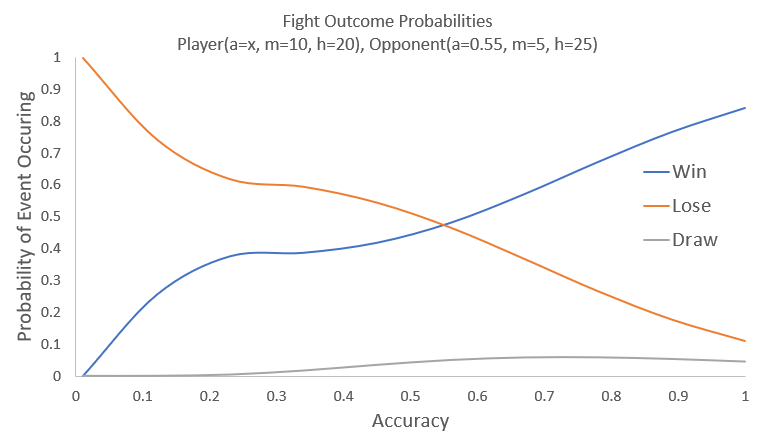
\includegraphics[width=\linewidth]{img/combat/fight_outcome_probabilities.png}
		\caption{
			The probability of the player winning, losing, and drawing during their fight with an opponent. Both are using the standard weapon distribution. The player's accuracy is varied which shows that the player needs at least 55\% accuracy to have a higher chance of winning than their opponent. With 0\% accuracy the player is guaranteed to lose, but with 100\% accuracy there is still a chance the opponent wins.
		}
		\label{fig:fight_outcome_probabilities}
	\end{figure}


	\begin{figure}
		\centering
		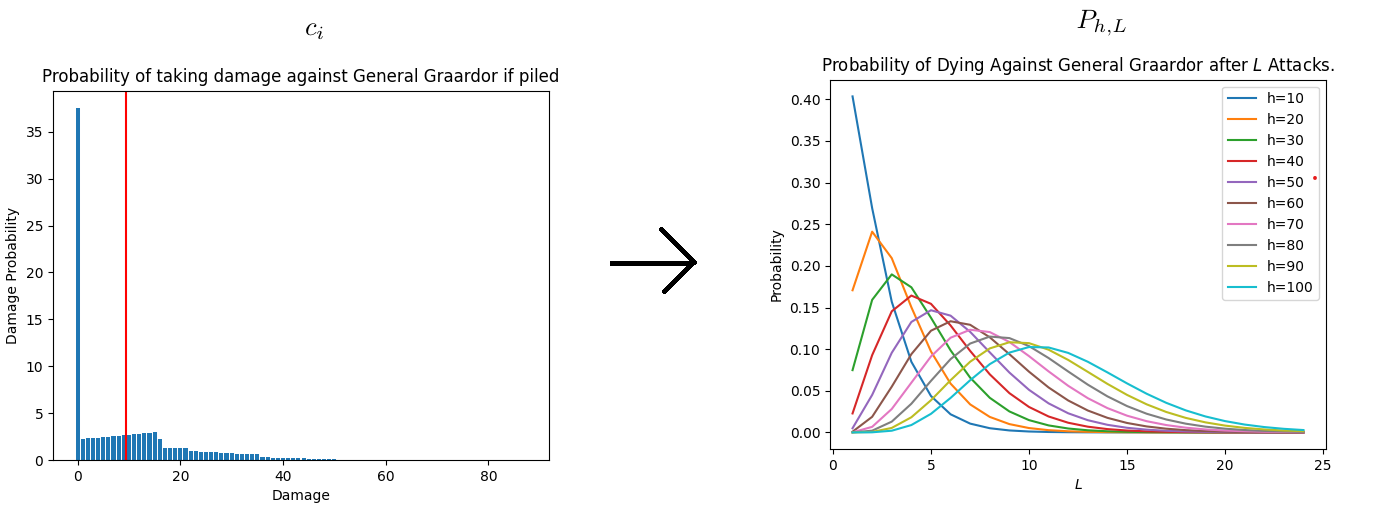
\includegraphics[width=\linewidth]{img/combat/bandos_slim.png}
		\caption{
			The damage distribution of \href{https://oldschool.runescape.wiki/w/General_Graardor}{General Graardor} (plus minions) assuming protect from melee (the average is in red). Under the mechanics of Eq.~(\ref{eq:p_h_l}), the probability of dying after L attacks is shown for different starting hitpoints. Near 0hp the player is expected to loss immediately. After about 50hp, it becomes impossible to get killed in one shot, and we get a Gaussian survival probability.
		}
		\label{fig:bandos}
	\end{figure}


	\begin{figure}
		\centering
		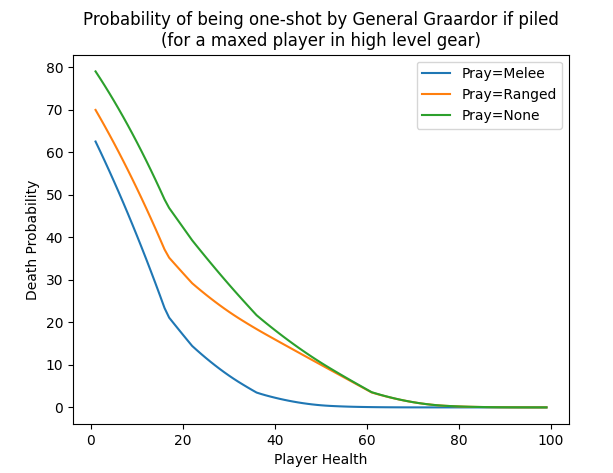
\includegraphics[width=\linewidth]{img/combat/bandos_one_shot.png}
		\caption{
			The best protection is melee regardless of player health. Over 80hp, it doesn't matter what you pray - you cannot be one shot. Just below that, if you are not praying melee you might get one-shot and range pray doesn't help you. If you are below 50hp, then you might get one-shot by ranged and so that prayer starts to matter again.
		}
		\label{fig:bandos_one_shot}
	\end{figure}